\documentclass{standalone}
\usepackage{tikz}
\usetikzlibrary{patterns, positioning}

\begin{document}
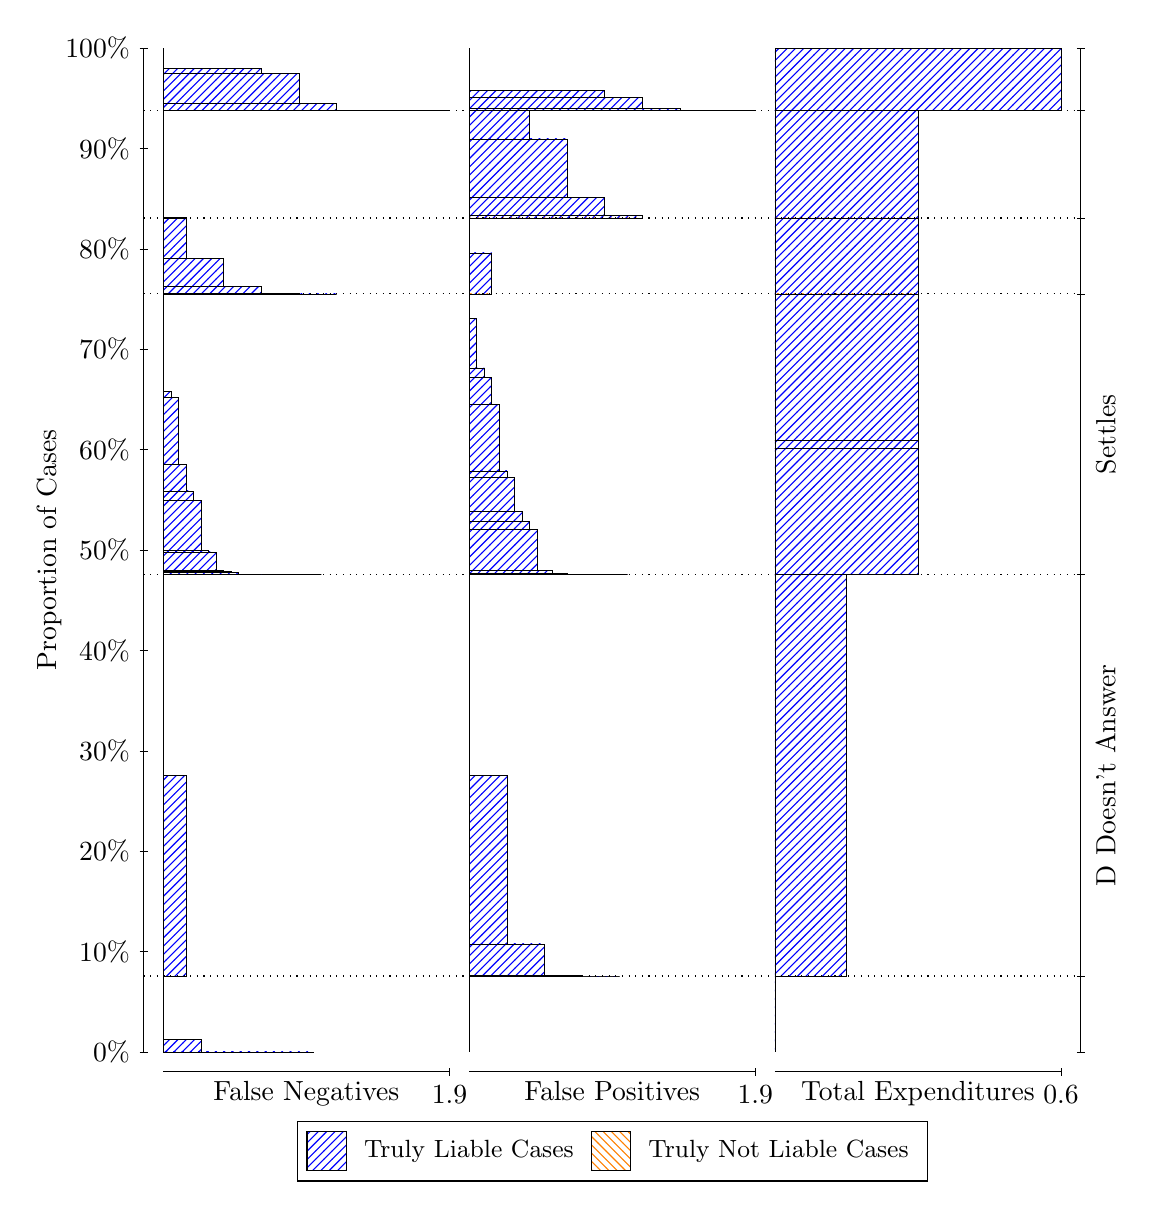
\begin{tikzpicture}
\draw[black, very thin] (1.5,1.75) -- (1.5,14.5);
\node[rotate=90, anchor=center] at (0.3, 8.125) {Proportion of Cases};
\draw[black, very thin] (1.45,1.75) -- (1.55,1.75);
\node[anchor=east] at (1.45, 1.75) {0\%};
\draw[black, very thin] (1.45,3.025) -- (1.55,3.025);
\node[anchor=east] at (1.45, 3.025) {10\%};
\draw[black, very thin] (1.45,4.3) -- (1.55,4.3);
\node[anchor=east] at (1.45, 4.3) {20\%};
\draw[black, very thin] (1.45,5.575) -- (1.55,5.575);
\node[anchor=east] at (1.45, 5.575) {30\%};
\draw[black, very thin] (1.45,6.85) -- (1.55,6.85);
\node[anchor=east] at (1.45, 6.85) {40\%};
\draw[black, very thin] (1.45,8.125) -- (1.55,8.125);
\node[anchor=east] at (1.45, 8.125) {50\%};
\draw[black, very thin] (1.45,9.4) -- (1.55,9.4);
\node[anchor=east] at (1.45, 9.4) {60\%};
\draw[black, very thin] (1.45,10.675) -- (1.55,10.675);
\node[anchor=east] at (1.45, 10.675) {70\%};
\draw[black, very thin] (1.45,11.95) -- (1.55,11.95);
\node[anchor=east] at (1.45, 11.95) {80\%};
\draw[black, very thin] (1.45,13.225) -- (1.55,13.225);
\node[anchor=east] at (1.45, 13.225) {90\%};
\draw[black, very thin] (1.45,14.5) -- (1.55,14.5);
\node[anchor=east] at (1.45, 14.5) {100\%};

\draw[black, very thin] (13.4,1.75) -- (13.4,14.5);
\draw[black, very thin] (13.35,1.75) -- (13.45,1.75);
\node[anchor=west] at (13.35, 1.75) {};
\draw[black, very thin] (13.35,2.7149) -- (13.45,2.7149);
\node[anchor=west] at (13.35, 2.7149) {};
\draw[black, very thin] (13.35,7.8133) -- (13.45,7.8133);
\node[anchor=west] at (13.35, 7.8133) {};
\draw[black, very thin] (13.35,11.379) -- (13.45,11.379);
\node[anchor=west] at (13.35, 11.379) {};
\draw[black, very thin] (13.35,12.342) -- (13.45,12.342);
\node[anchor=west] at (13.35, 12.342) {};
\draw[black, very thin] (13.35,13.708) -- (13.45,13.708);
\node[anchor=west] at (13.35, 13.708) {};
\draw[black, very thin] (13.35,14.5) -- (13.45,14.5);
\node[anchor=west] at (13.35, 14.5) {};

\draw[black, very thin, pattern color=blue, pattern=north east lines] (1.75,1.75) rectangle (3.6623,1.75);
\draw[black, very thin, pattern color=blue, pattern=north east lines] (1.75,1.75) rectangle (3.1842,1.75);
\draw[black, very thin, pattern color=blue, pattern=north east lines] (1.75,1.75) rectangle (2.7061,1.7514);
\draw[black, very thin, pattern color=blue, pattern=north east lines] (1.75,1.7514) rectangle (2.2281,1.908);
\draw[black, very thin, pattern color=orange, pattern=north west lines] (1.75,1.908) rectangle (1.75,1.908);
\draw[black, very thin, pattern color=blue, pattern=north east lines] (1.75,1.908) rectangle (1.75,2.7149);
\draw[black, very thin, pattern color=blue, pattern=north east lines] (1.75,2.7149) rectangle (2.0368,5.2608);
\draw[black, very thin, pattern color=orange, pattern=north west lines] (1.75,5.2608) rectangle (1.75,5.2608);
\draw[black, very thin, pattern color=blue, pattern=north east lines] (1.75,5.2608) rectangle (1.75,7.8133);
\draw[black, very thin, pattern color=blue, pattern=north east lines] (1.75,7.8133) rectangle (3.7579,7.8133);
\draw[black, very thin, pattern color=blue, pattern=north east lines] (1.75,7.8133) rectangle (3.5667,7.8133);
\draw[black, very thin, pattern color=blue, pattern=north east lines] (1.75,7.8133) rectangle (3.3754,7.8133);
\draw[black, very thin, pattern color=blue, pattern=north east lines] (1.75,7.8133) rectangle (3.2798,7.8133);
\draw[black, very thin, pattern color=blue, pattern=north east lines] (1.75,7.8133) rectangle (3.1842,7.8133);
\draw[black, very thin, pattern color=blue, pattern=north east lines] (1.75,7.8133) rectangle (3.0886,7.8133);
\draw[black, very thin, pattern color=blue, pattern=north east lines] (1.75,7.8133) rectangle (2.993,7.8133);
\draw[black, very thin, pattern color=blue, pattern=north east lines] (1.75,7.8133) rectangle (2.8974,7.8176);
\draw[black, very thin, pattern color=blue, pattern=north east lines] (1.75,7.8176) rectangle (2.8018,7.8178);
\draw[black, very thin, pattern color=blue, pattern=north east lines] (1.75,7.8178) rectangle (2.7061,7.8419);
\draw[black, very thin, pattern color=blue, pattern=north east lines] (1.75,7.8419) rectangle (2.6105,7.8419);
\draw[black, very thin, pattern color=blue, pattern=north east lines] (1.75,7.8419) rectangle (2.6105,7.8505);
\draw[black, very thin, pattern color=blue, pattern=north east lines] (1.75,7.8505) rectangle (2.5149,7.8662);
\draw[black, very thin, pattern color=blue, pattern=north east lines] (1.75,7.8662) rectangle (2.4193,8.1009);
\draw[black, very thin, pattern color=blue, pattern=north east lines] (1.75,8.1009) rectangle (2.3237,8.1009);
\draw[black, very thin, pattern color=blue, pattern=north east lines] (1.75,8.1009) rectangle (2.3237,8.1213);
\draw[black, very thin, pattern color=blue, pattern=north east lines] (1.75,8.1213) rectangle (2.2281,8.7534);
\draw[black, very thin, pattern color=blue, pattern=north east lines] (1.75,8.7534) rectangle (2.1325,8.7534);
\draw[black, very thin, pattern color=blue, pattern=north east lines] (1.75,8.7534) rectangle (2.1325,8.876);
\draw[black, very thin, pattern color=blue, pattern=north east lines] (1.75,8.876) rectangle (2.0368,9.2156);
\draw[black, very thin, pattern color=blue, pattern=north east lines] (1.75,9.2156) rectangle (1.9412,10.062);
\draw[black, very thin, pattern color=blue, pattern=north east lines] (1.75,10.062) rectangle (1.9412,10.062);
\draw[black, very thin, pattern color=blue, pattern=north east lines] (1.75,10.062) rectangle (1.8456,10.062);
\draw[black, very thin, pattern color=blue, pattern=north east lines] (1.75,10.062) rectangle (1.8456,10.142);
\draw[black, very thin, pattern color=blue, pattern=north east lines] (1.75,10.142) rectangle (1.75,10.142);
\draw[black, very thin, pattern color=orange, pattern=north west lines] (1.75,10.142) rectangle (1.75,10.142);
\draw[black, very thin, pattern color=blue, pattern=north east lines] (1.75,10.142) rectangle (1.75,11.379);
\draw[black, very thin, pattern color=blue, pattern=north east lines] (1.75,11.379) rectangle (3.9491,11.379);
\draw[black, very thin, pattern color=blue, pattern=north east lines] (1.75,11.379) rectangle (3.4711,11.38);
\draw[black, very thin, pattern color=blue, pattern=north east lines] (1.75,11.38) rectangle (2.993,11.468);
\draw[black, very thin, pattern color=blue, pattern=north east lines] (1.75,11.468) rectangle (2.5149,11.824);
\draw[black, very thin, pattern color=blue, pattern=north east lines] (1.75,11.824) rectangle (2.0368,12.342);
\draw[black, very thin, pattern color=orange, pattern=north west lines] (1.75,12.342) rectangle (1.75,12.342);
\draw[black, very thin, pattern color=blue, pattern=north east lines] (1.75,12.342) rectangle (2.0368,12.346);
\draw[black, very thin, pattern color=orange, pattern=north west lines] (1.75,12.346) rectangle (1.75,12.346);
\draw[black, very thin, pattern color=blue, pattern=north east lines] (1.75,12.346) rectangle (1.75,13.708);
\draw[black, very thin, pattern color=blue, pattern=north east lines] (1.75,13.708) rectangle (5.3833,13.708);
\draw[black, very thin, pattern color=blue, pattern=north east lines] (1.75,13.708) rectangle (4.9053,13.708);
\draw[black, very thin, pattern color=blue, pattern=north east lines] (1.75,13.708) rectangle (4.4272,13.71);
\draw[black, very thin, pattern color=blue, pattern=north east lines] (1.75,13.71) rectangle (3.9491,13.797);
\draw[black, very thin, pattern color=blue, pattern=north east lines] (1.75,13.797) rectangle (3.4711,14.179);
\draw[black, very thin, pattern color=blue, pattern=north east lines] (1.75,14.179) rectangle (2.993,14.246);
\draw[black, very thin, pattern color=blue, pattern=north east lines] (1.75,14.246) rectangle (2.6105,14.246);
\draw[black, very thin, pattern color=blue, pattern=north east lines] (1.75,14.246) rectangle (2.5149,14.246);
\draw[black, very thin, pattern color=blue, pattern=north east lines] (1.75,14.246) rectangle (2.1325,14.246);
\draw[black, very thin, pattern color=orange, pattern=north west lines] (1.75,14.246) rectangle (1.75,14.246);
\draw[black, very thin, pattern color=blue, pattern=north east lines] (1.75,14.246) rectangle (1.75,14.5);
\draw[black, very thin, pattern color=orange, pattern=north west lines] (5.6333,1.75) rectangle (5.6333,1.75);
\draw[black, very thin, pattern color=blue, pattern=north east lines] (5.6333,1.75) rectangle (5.6333,2.7149);
\draw[black, very thin, pattern color=orange, pattern=north west lines] (5.6333,2.7149) rectangle (7.5456,2.7149);
\draw[black, very thin, pattern color=blue, pattern=north east lines] (5.6333,2.7149) rectangle (7.5456,2.7149);
\draw[black, very thin, pattern color=blue, pattern=north east lines] (5.6333,2.7149) rectangle (7.0675,2.7182);
\draw[black, very thin, pattern color=blue, pattern=north east lines] (5.6333,2.7182) rectangle (6.5895,3.1225);
\draw[black, very thin, pattern color=blue, pattern=north east lines] (5.6333,3.1225) rectangle (6.1114,5.2674);
\draw[black, very thin, pattern color=blue, pattern=north east lines] (5.6333,5.2674) rectangle (5.6333,7.8133);
\draw[black, very thin, pattern color=orange, pattern=north west lines] (5.6333,7.8133) rectangle (7.6412,7.8133);
\draw[black, very thin, pattern color=blue, pattern=north east lines] (5.6333,7.8133) rectangle (7.6412,7.8133);
\draw[black, very thin, pattern color=orange, pattern=north west lines] (5.6333,7.8133) rectangle (7.45,7.8133);
\draw[black, very thin, pattern color=blue, pattern=north east lines] (5.6333,7.8133) rectangle (7.45,7.8133);
\draw[black, very thin, pattern color=orange, pattern=north west lines] (5.6333,7.8133) rectangle (7.2588,7.8133);
\draw[black, very thin, pattern color=blue, pattern=north east lines] (5.6333,7.8133) rectangle (7.2588,7.8133);
\draw[black, very thin, pattern color=blue, pattern=north east lines] (5.6333,7.8133) rectangle (7.1632,7.8133);
\draw[black, very thin, pattern color=orange, pattern=north west lines] (5.6333,7.8133) rectangle (7.0675,7.8133);
\draw[black, very thin, pattern color=blue, pattern=north east lines] (5.6333,7.8133) rectangle (7.0675,7.8133);
\draw[black, very thin, pattern color=blue, pattern=north east lines] (5.6333,7.8133) rectangle (6.9719,7.8133);
\draw[black, very thin, pattern color=orange, pattern=north west lines] (5.6333,7.8133) rectangle (6.8763,7.8133);
\draw[black, very thin, pattern color=blue, pattern=north east lines] (5.6333,7.8133) rectangle (6.8763,7.825);
\draw[black, very thin, pattern color=blue, pattern=north east lines] (5.6333,7.825) rectangle (6.7807,7.825);
\draw[black, very thin, pattern color=orange, pattern=north west lines] (5.6333,7.825) rectangle (6.6851,7.825);
\draw[black, very thin, pattern color=blue, pattern=north east lines] (5.6333,7.825) rectangle (6.6851,7.8702);
\draw[black, very thin, pattern color=orange, pattern=north west lines] (5.6333,7.8702) rectangle (6.6851,7.8702);
\draw[black, very thin, pattern color=blue, pattern=north east lines] (5.6333,7.8702) rectangle (6.6851,7.8702);
\draw[black, very thin, pattern color=blue, pattern=north east lines] (5.6333,7.8702) rectangle (6.5895,7.8702);
\draw[black, very thin, pattern color=blue, pattern=north east lines] (5.6333,7.8702) rectangle (6.4939,7.8702);
\draw[black, very thin, pattern color=orange, pattern=north west lines] (5.6333,7.8702) rectangle (6.4939,7.8702);
\draw[black, very thin, pattern color=blue, pattern=north east lines] (5.6333,7.8702) rectangle (6.4939,8.3855);
\draw[black, very thin, pattern color=blue, pattern=north east lines] (5.6333,8.3855) rectangle (6.3982,8.4878);
\draw[black, very thin, pattern color=orange, pattern=north west lines] (5.6333,8.4878) rectangle (6.3026,8.4878);
\draw[black, very thin, pattern color=blue, pattern=north east lines] (5.6333,8.4878) rectangle (6.3026,8.6178);
\draw[black, very thin, pattern color=blue, pattern=north east lines] (5.6333,8.6178) rectangle (6.207,9.0503);
\draw[black, very thin, pattern color=blue, pattern=north east lines] (5.6333,9.0503) rectangle (6.207,9.0503);
\draw[black, very thin, pattern color=orange, pattern=north west lines] (5.6333,9.0503) rectangle (6.1114,9.0503);
\draw[black, very thin, pattern color=blue, pattern=north east lines] (5.6333,9.0503) rectangle (6.1114,9.1301);
\draw[black, very thin, pattern color=blue, pattern=north east lines] (5.6333,9.1301) rectangle (6.0158,9.1301);
\draw[black, very thin, pattern color=blue, pattern=north east lines] (5.6333,9.1301) rectangle (6.0158,9.9767);
\draw[black, very thin, pattern color=blue, pattern=north east lines] (5.6333,9.9767) rectangle (5.9202,10.316);
\draw[black, very thin, pattern color=blue, pattern=north east lines] (5.6333,10.316) rectangle (5.8246,10.439);
\draw[black, very thin, pattern color=blue, pattern=north east lines] (5.6333,10.439) rectangle (5.7289,11.071);
\draw[black, very thin, pattern color=blue, pattern=north east lines] (5.6333,11.071) rectangle (5.7289,11.071);
\draw[black, very thin, pattern color=blue, pattern=north east lines] (5.6333,11.071) rectangle (5.6333,11.379);
\draw[black, very thin, pattern color=orange, pattern=north west lines] (5.6333,11.379) rectangle (5.9202,11.379);
\draw[black, very thin, pattern color=blue, pattern=north east lines] (5.6333,11.379) rectangle (5.9202,11.897);
\draw[black, very thin, pattern color=blue, pattern=north east lines] (5.6333,11.897) rectangle (5.6333,12.342);
\draw[black, very thin, pattern color=orange, pattern=north west lines] (5.6333,12.342) rectangle (7.8325,12.342);
\draw[black, very thin, pattern color=blue, pattern=north east lines] (5.6333,12.342) rectangle (7.8325,12.376);
\draw[black, very thin, pattern color=blue, pattern=north east lines] (5.6333,12.376) rectangle (7.3544,12.605);
\draw[black, very thin, pattern color=blue, pattern=north east lines] (5.6333,12.605) rectangle (6.8763,13.346);
\draw[black, very thin, pattern color=blue, pattern=north east lines] (5.6333,13.346) rectangle (6.3982,13.704);
\draw[black, very thin, pattern color=blue, pattern=north east lines] (5.6333,13.704) rectangle (5.9202,13.708);
\draw[black, very thin, pattern color=orange, pattern=north west lines] (5.6333,13.708) rectangle (9.2667,13.708);
\draw[black, very thin, pattern color=blue, pattern=north east lines] (5.6333,13.708) rectangle (9.2667,13.708);
\draw[black, very thin, pattern color=orange, pattern=north west lines] (5.6333,13.708) rectangle (8.7886,13.708);
\draw[black, very thin, pattern color=blue, pattern=north east lines] (5.6333,13.708) rectangle (8.7886,13.709);
\draw[black, very thin, pattern color=orange, pattern=north west lines] (5.6333,13.709) rectangle (8.3105,13.709);
\draw[black, very thin, pattern color=blue, pattern=north east lines] (5.6333,13.709) rectangle (8.3105,13.729);
\draw[black, very thin, pattern color=orange, pattern=north west lines] (5.6333,13.729) rectangle (7.8325,13.729);
\draw[black, very thin, pattern color=blue, pattern=north east lines] (5.6333,13.729) rectangle (7.8325,13.878);
\draw[black, very thin, pattern color=blue, pattern=north east lines] (5.6333,13.878) rectangle (7.3544,13.959);
\draw[black, very thin, pattern color=blue, pattern=north east lines] (5.6333,13.959) rectangle (6.8763,13.962);
\draw[black, very thin, pattern color=blue, pattern=north east lines] (5.6333,13.962) rectangle (6.3982,13.962);
\draw[black, very thin, pattern color=orange, pattern=north west lines] (5.6333,13.962) rectangle (6.0158,13.962);
\draw[black, very thin, pattern color=blue, pattern=north east lines] (5.6333,13.962) rectangle (6.0158,13.963);
\draw[black, very thin, pattern color=blue, pattern=north east lines] (5.6333,13.963) rectangle (5.9202,13.963);
\draw[black, very thin, pattern color=orange, pattern=north west lines] (5.6333,13.963) rectangle (5.6333,13.963);
\draw[black, very thin, pattern color=blue, pattern=north east lines] (5.6333,13.963) rectangle (5.6333,14.5);
\draw[black, very thin, pattern color=orange, pattern=north west lines] (9.5167,1.75) rectangle (9.5167,1.75);
\draw[black, very thin, pattern color=blue, pattern=north east lines] (9.5167,1.75) rectangle (9.5167,2.7149);
\draw[black, very thin, pattern color=orange, pattern=north west lines] (9.5167,2.7149) rectangle (10.425,2.7149);
\draw[black, very thin, pattern color=blue, pattern=north east lines] (9.5167,2.7149) rectangle (10.425,7.8133);
\draw[black, very thin, pattern color=orange, pattern=north west lines] (9.5167,7.8133) rectangle (11.333,7.8133);
\draw[black, very thin, pattern color=blue, pattern=north east lines] (9.5167,7.8133) rectangle (11.333,9.4166);
\draw[black, very thin, pattern color=orange, pattern=north west lines] (9.5167,9.4166) rectangle (11.333,9.4166);
\draw[black, very thin, pattern color=blue, pattern=north east lines] (9.5167,9.4166) rectangle (11.333,9.5169);
\draw[black, very thin, pattern color=orange, pattern=north west lines] (9.5167,9.5169) rectangle (11.333,9.5169);
\draw[black, very thin, pattern color=blue, pattern=north east lines] (9.5167,9.5169) rectangle (11.333,11.379);
\draw[black, very thin, pattern color=orange, pattern=north west lines] (9.5167,11.379) rectangle (11.333,11.379);
\draw[black, very thin, pattern color=blue, pattern=north east lines] (9.5167,11.379) rectangle (11.333,12.342);
\draw[black, very thin, pattern color=orange, pattern=north west lines] (9.5167,12.342) rectangle (11.333,12.342);
\draw[black, very thin, pattern color=blue, pattern=north east lines] (9.5167,12.342) rectangle (11.333,13.708);
\draw[black, very thin, pattern color=orange, pattern=north west lines] (9.5167,13.708) rectangle (13.15,13.708);
\draw[black, very thin, pattern color=blue, pattern=north east lines] (9.5167,13.708) rectangle (13.15,14.5);
\draw[black, dotted] (1.5,2.7149) -- (13.4,2.7149);
\draw[black, dotted] (1.5,7.8133) -- (13.4,7.8133);
\draw[black, dotted] (1.5,11.379) -- (13.4,11.379);
\draw[black, dotted] (1.5,12.342) -- (13.4,12.342);
\draw[black, dotted] (1.5,13.708) -- (13.4,13.708);
\draw[black, very thin] (1.75,1.5) -- (5.3833,1.5);
\node[anchor=north] at (3.5667, 1.5) {False Negatives};
\draw[black, very thin] (5.3833,1.45) -- (5.3833,1.55);
\node[anchor=north] at (5.3833, 1.45) {1.9};

\draw[black, very thin] (5.6333,1.5) -- (9.2667,1.5);
\node[anchor=north] at (7.45, 1.5) {False Positives};
\draw[black, very thin] (9.2667,1.45) -- (9.2667,1.55);
\node[anchor=north] at (9.2667, 1.45) {1.9};

\draw[black, very thin] (9.5167,1.5) -- (13.15,1.5);
\node[anchor=north] at (11.333, 1.5) {Total Expenditures};
\draw[black, very thin] (13.15,1.45) -- (13.15,1.55);
\node[anchor=north] at (13.15, 1.45) {0.6};


\node[black, centered, rotate=90] at (13.72, 5.2641) {D Doesn't Answer};
\node[black, centered, rotate=90] at (13.72, 9.5961) {Settles};




\draw (7.449999999999999,1.5) node[draw=none] (baseCoordinate) {};
\begin{scope}[align=center]
        \matrix[scale=0.5, draw=black, below=0.5cm of baseCoordinate, nodes={draw}, column sep=0.1cm]{
            \node[rectangle, draw, minimum width=0.5cm, minimum height=0.5cm, pattern=north east lines, pattern color=blue] {}; &
            \node[draw=none, font=\small] (B) {Truly Liable Cases}; &
            \node[rectangle, draw, minimum width=0.5cm, minimum height=0.5cm, pattern=north west lines, pattern color=orange] {}; &
            \node[draw=none, font=\small] (B) {Truly Not Liable Cases}; \\
            };
\end{scope}

\end{tikzpicture}
\end{document}